\section{Reliability Alignment}

In this section, we introduce the alignment framework for tool reliability, Relign. As illustrated in Figure 1, Relign consists of three components: the tool-level alignment objectives (\ref{3.1}), the process for synthesizing tool preference data(\ref{3.2}), and the overall training pipeline (\ref{3.2}). We identify the primary cause of tool hallucinations as the model's lack of proper modeling of the decision conditions when making tool-related decisions. Specifically, if an LLM calls a tool under conditions where the decision criteria are not met—such as when the tool's parameters are unknown or when the tool is mismatched with the task—the occurrence of tool hallucinations significantly increases. To address this, we introduce the concept of \textit{indecisive action space}, where alternative actions such as \texttt{ChangeTools} and \texttt{TalkToUser}  when tool invocation conditions are unmet. Furthermore, we enhance the model's awareness of boundary conditions in tool calling by training it with synthesized alignment data.

\begin{figure*}[t!]
    \centering
    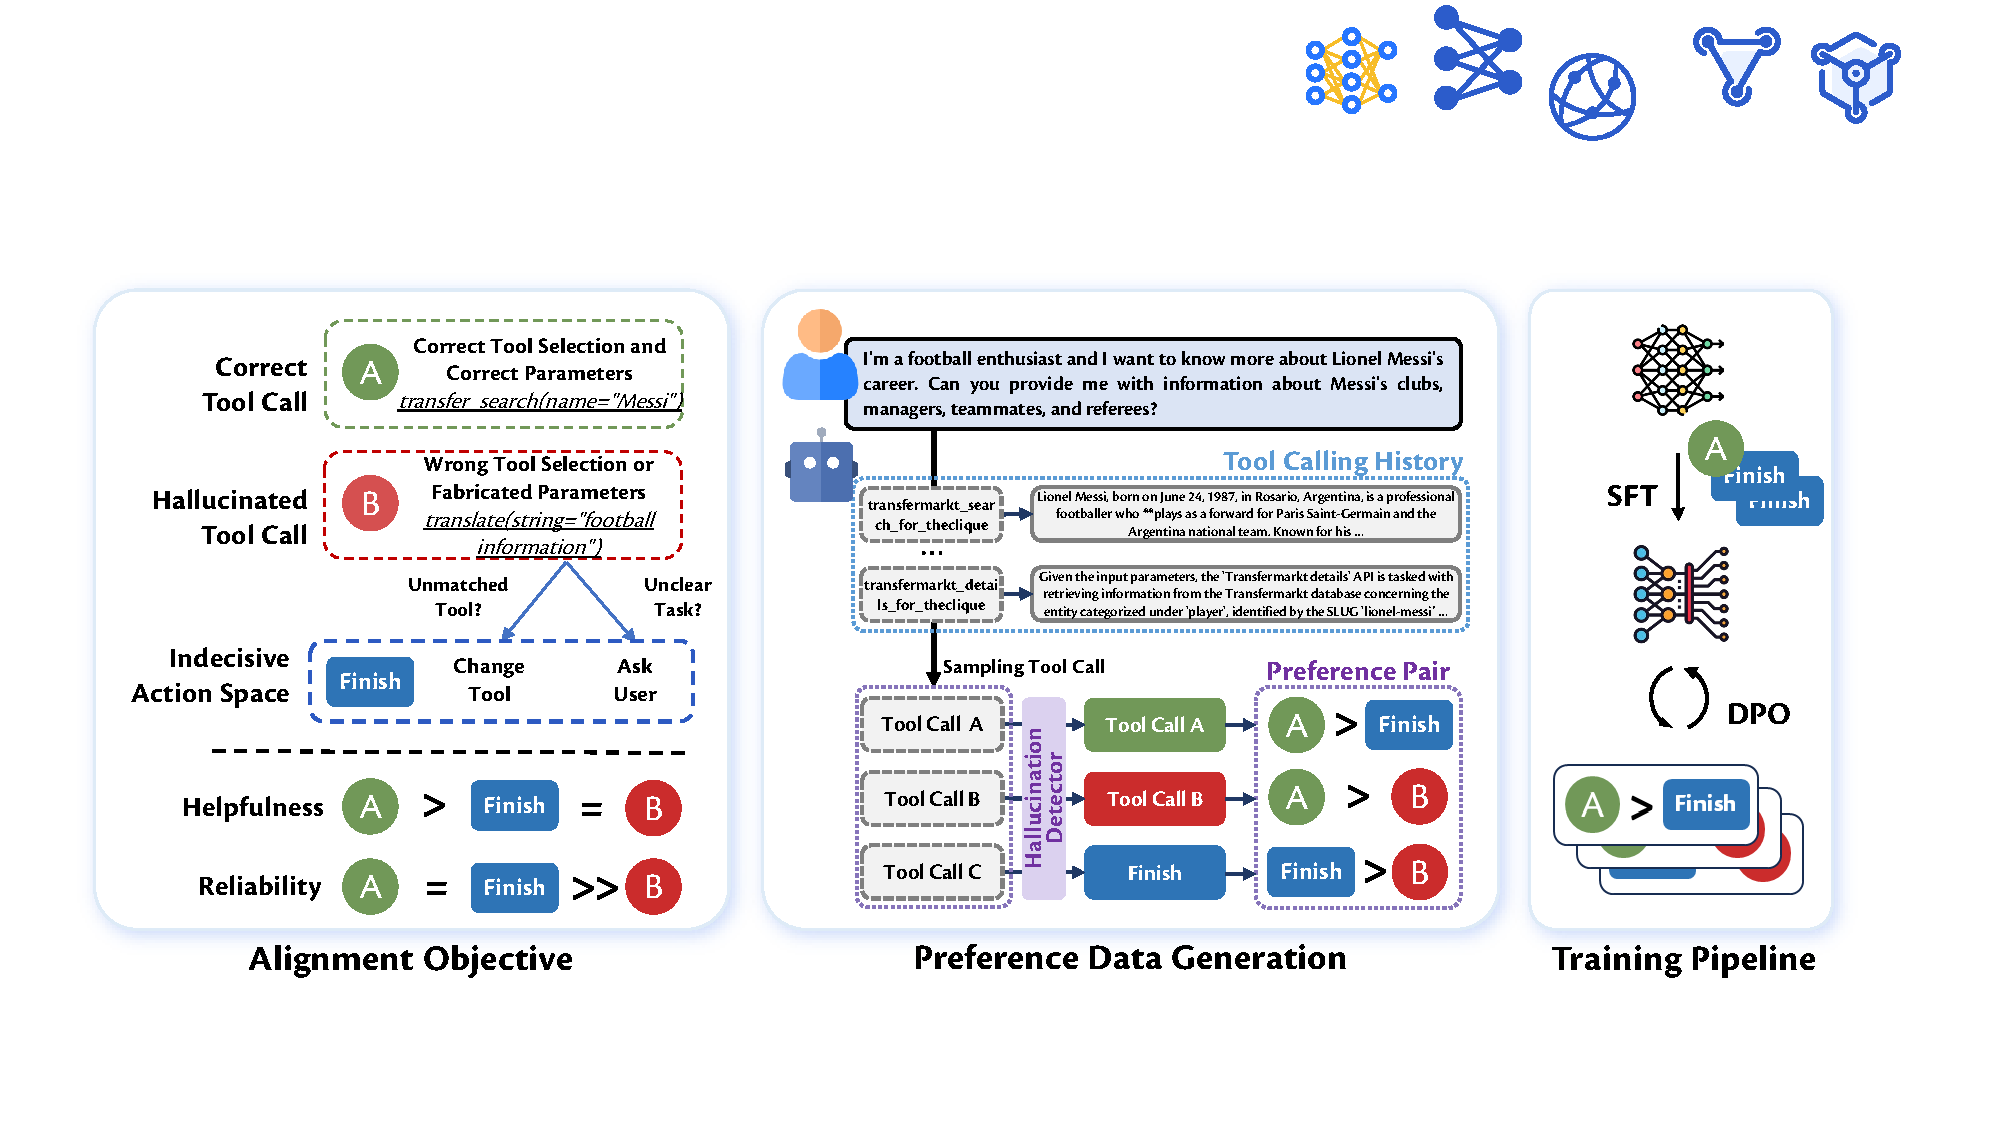
\includegraphics[width=\linewidth,trim=40 70 70 120,clip]{figs/system.pdf}
    \vspace{-6mm}
    \caption{\textbf{The system illustration of Relign.}} 
    \vspace{-4mm}
    \label{fig:system}
\end{figure*}

\subsection{Alignment Goal}
\label{3.1}
% \paragraph{Task-Level Preference Hierarchy}
% At the task completion level, we establish a strict preference ordering based on outcome quality:
% \begin{itemize}
%     \item \textbf{Successful trajectories} ($T_{\text{success}}$) that achieve accurate task completion through valid tool calls are maximally preferred
%     \item \textbf{Aborted trajectories} ($T_{\text{abort}}$) where the model actively terminates execution via indecisive actions (e.g., "Insufficient information to proceed") are intermediately preferred
%     \item \textbf{Hallucinated trajectories} ($T_{\text{hallucination}}$) containing invalid tool calls are strictly penalized
% \end{itemize}

% Formally, this hierarchy satisfies:
% \begin{equation}
%     T_{\text{success}} > T_{\text{abort}} > T_{\text{hallucination}}
% \end{equation}


% 
The alignment goal for reliable tool calling in LLMs focuses on ensuring accurate and effective interactions with external tools throughout the task completion process. From a task perspective, the primary objective is to maximize successful tool calling while minimizing hallucinations. This can be formalized as a preference hierarchy: formally, let $T$ represent a tool calling trajectory, and $H(T)$ the hallucination rate within that trajectory. For a given task, we define the alignment preference as:
$$
T_{\text{success}} > T_{\text{failure}} > T_{\text{hallucination}},
$$
where $T_{\text{success}}$ represents a successful trajectory, $T_{\text{failure}}$ represents a trajectory resulting in task failure or abandonment, and $T_{\text{hallucination}}$ represents a trajectory that generates a hallucinated result.

In our experiments, we observe that when a model exhibits a high rate of tool hallucinations, it tends to favor producing hallucinated outputs rather than acknowledging failure. This behavior poses a significant risk, as hallucinated results may mislead users into believing the task was successfully completed, thus undermining trust in the system.


Therefore, building upon the task-level alignment preference, we define the alignment preference at step level for tool interaction tasks. Specifically, a non-hallucinated tool call is preferred over indecisive actions and hallucinated tool calls. This preference hierarchy can be formalized as:
$$
A_{\text{correct}} > A_{\text{indecisive}} > A_{\text{hallcuinated}},
$$
where $A_{\text{correct}}$, $A_{\text{indecisive}}$, $A_{\text{hallcuinated}}$ represent correct tool calling actions, indecisive actions and hallucinated tool calling actions, respectively. We also find that for many tasks, the number of required tool callings is typically fixed. Models that invoke tools excessively tend to introduce more hallucinations. Thus, minimizing tool hallucination not only improves task reliability but also reduces the overall number of tool callings, leading to more efficient tool usage. 



\subsection{Alignment Methods}
\label{3.2}
The overall data synthesis and alignment training process is illustrated in the middle and right parts of Figure 4. First, we construct reliable supervision data for Supervised Fine-Tuning (SFT) to train the model on the appropriate use of indecisive actions. After the initial SFT training, we sample and synthesize reliable preference data based on the model, which is then used to further train the model through the Direct Preference Optimization (DPO) approach. This two-step process ensures that the model not only learns to handle indecisive actions effectively but also aligns with the desired task-level preferences in the long run.

\subsubsection{Reliable SFT}

% The first step in our approach is Supervised Fine-Tuning (SFT), where we sample tool calling traces for specific tasks. If any of these traces lead to successful task completion, we select those with the fewest hallucinations as the labels for fine-tuning. If all sampled traces fail, we consider that the task might be infeasible for the model and design strategies for rejection based on the hallucination types. Specifically:

% \begin{itemize}
% \item \textbf{Tool Type Hallucinations:} When these types of hallucinations occur, indicating that the available tools are insufficient for the task, the model is trained to trigger a “ChangeTools” function, requesting alternative tools.
% \item \textbf{Tool Content Hallucinations:} If hallucinations are due to incorrect tool content, the model learns to invoke a “TalkToUser” function, signaling task completion through communication.
% \end{itemize}

We observe that among the four types of hallucinations, tool type and content hallucinations occur more frequently. Therefore, the main objective of our Supervised Fine-Tuning (SFT) is to train the model to address these hallucinations by learning to invoke "ChangeTools" for tool type hallucinations and "TalkToUser" for tool content hallucinations. Similar to the data synthesis in RelyToolBench, we select specific samples from ToolBench's training data, modifying them by replacing tool sets or removing tool parameters to simulate these hallucinations. The model is then trained to output the appropriate actions based on these modifications. To ensure the generalizability of the experiment and results, the training data we selected involves only a single tool.

\subsubsection{Reliable DPO}

After obtaining a model capable of outputting indecisive actions through SFT, we further optimize it using Direct Preference Optimization (DPO). Direct Preference Optimization (DPO) focuses on constructing preference data to fine-tune the model’s behavior. The goal of DPO is to guide the model in selecting optimal tool calling traces based on task success and hallucination types. Specifically, for each tool calling trajectory, at any given step, we sample multiple responses and use a hallucination evaluator to categorize these responses into three types: hallucinated tool calling action $A_{hallucinated}$, non-hallucinated tool calling action $A_{coreect}$, and indecisive actions $A_{indecisive}$. Based on these classifications, we generate three types of preference pairs: $(A_{correct}>A_{indecisive})$, $(A_{indecisive}>A_{hallucinated})$, $(A_{correct}>A_{hallucinated})$. For each type of preference pair, we randomly select one from the sampled responses to construct the DPO training data.
% We define preference data across three main scenarios, which dictate how the model ranks different responses:

% \begin{itemize}
% \item \textbf{Successful vs. Unsuccessful Traces:} If there are successful traces for a task, traces with fewer hallucinations are preferred over those with more hallucinations. Additionally, successful traces are always preferred over traces where the model invokes rejection mechanisms such as tool changes or task abandonment.
% \item \textbf{Tool Type Hallucinations:} When the primary hallucination type is tool relevance (i.e., the model incorrectly selects irrelevant tools), traces where the model invokes a “ChangeTools” function are preferred over traces where it persists with hallucinated tool calls.
% \item \textbf{Tool Content Hallucinations:} If the hallucinations are due to incorrect tool content (i.e., the model generates incorrect output based on the tool’s response), traces where the model communicates task difficulties via the “TalkToUser” function are preferred over those that continue using incorrect tool data.
% \end{itemize}

% The ranking preferences can be summarized as:
% $$
% T_{s, l} \succ T_{s, h} \succ T_{f,c} = T_{f, t} \succ T_{f, h},
% $$
% where $T_{s, l}$ and $T_{s, h}$ represent the successful trajectory with relatively low and high tool hallucinations, respectively; $T_{f,c}$ and $T_{f,t}$ represent unsuccessful trajectories where rejection mechanisms with “ChangeTools” and “TalkToUser” function were employed; these are preferred over $T_{f,h}$ with high tool hallucinations or lead to hallucinated outcomes.

The DPO framework ensures that the model learns to rank trajectories according to these preferences. By optimizing over such data, the model becomes capable of choosing the most reliable tool calling sequence or recognizing when to abandon a task or seek further clarification from the user.

% \subsubsection{Joint Training of Reliable SFT and DPO}

% To ensure training stability and maximize model performance, we adopt two joint training strategies that integrate Supervised Fine-Tuning (SFT) and Direct Preference Optimization (DPO). The first approach involves a unified loss function where the losses from SFT and DPO are optimized simultaneously:

% $$
% L_{\text{total}} = \alpha L_{\text{SFT}} + \beta L_{\text{DPO}}.
% $$
 
% This simultaneous optimization stabilizes DPO while leveraging the supervised signals from SFT.

% The second approach involves a sequential process: we first train an SFT model, then sample data from it to generate DPO-specific training data. This allows DPO to build upon the strong foundation of the SFT model, further enhancing performance through preference-based fine-tuning. Both strategies aim to maximize the model’s ability to handle complex tasks, minimize hallucinations, and invoke appropriate rejection strategies.